\documentclass[notitlepage,aps,prd,nofootinbib]{revtex4-1}

\usepackage{subfig}
%\usepackage[colorinlistoftodos]{todonotes}
\usepackage{float}

%\usepackage[protrusion=true,expansion=true]{microtype}
\usepackage{amsmath}
\usepackage{amssymb}
\usepackage{bbm}
\usepackage{ulem}
%\usepackage{feynmp-auto}
%\usepackage{slashed}
%\usepackage[absolute,overlay]{textpos}
\usepackage[usenames, dvipsnames]{color}
\usepackage{graphicx}
\usepackage{subfigure}
\usepackage{listings}
\usepackage{epsfig}
\usepackage{hyperref}
%\usepackage{tikz}
\usepackage{enumerate}
%\usepackage{fixltx2e} % buggy
\usepackage[compatibility=false]{caption}
%\usepackage{subcaption} % doesn't work with subfigure
\usepackage{pdfpages}
%\usepackage{setspace}
\usepackage{verbatim}
\usepackage{physics}

% Turn off meaningless float warnings
\usepackage{silence}
\WarningFilter{revtex4-1}{Repair the float}

\DeclareRobustCommand{\orderof}{\ensuremath{\mathcal{O}}}

\definecolor{dukeblue}{RGB}{0,0,156}
\definecolor{dukedarkblue}{RGB}{0,26,87}
\definecolor{dukeblack}{RGB}{79,79,79}
\definecolor{dukegray}{RGB}{79,79,79}
\definecolor{dukesecbrown}{RGB}{217,200,158}
\definecolor{dukesecblue}{RGB}{127,169,174}

%\renewcommand*{\thefootnote}{\fnsymbol{footnote}}

%%%%%%%%%%%%%%%%%%%%%%%%%%%%%%%%%%%%%%%%%%%%%%%%%%%%%%%%%%%%%%%%%%%%%%%%%%%%%%%%%%%%%
\hypersetup{
    breaklinks,
    baseurl       = http://,
    pdfborder     = 0 0 0,
    pdfpagemode   = UseNone,% do not show thumbnails or bookmarks on opening
    pdfstartpage  = 1,
    bookmarksopen = true,
    bookmarksdepth= 2,% to show sections and subsections
% revtex needs author and title declared after \begin{document}, so have to hard code them...
%    pdfauthor     = {\@author},
%    pdftitle      = {\@title},
    pdfauthor     = {Yuanyuan Xu, Matthew Epland, Xiaqing Li, Wesley Cohen},
    pdftitle      = {Phys 566 Group Project 1},
    pdfsubject    = {},
    pdfkeywords   = {}}


% Code import settings
%%%%%%%%%%%%%%%%%%%%%%%%%%%%%%%%%%%%%%%%%%%%%%%%%%%%%%%%%%%%%%%%%%%%%%%%%%%%%%%%%%%%%
\definecolor{mygreen}{rgb}{0,0.6,0}
\definecolor{mygray}{rgb}{0.5,0.5,0.5}
\definecolor{mymauve}{rgb}{0.58,0,0.82}

%\lstset{ %
\lstdefinestyle{python}{ %
  backgroundcolor=\color{white},   % choose the background color; you must add \usepackage{color} or \usepackage{xcolor}
  basicstyle=\scriptsize,          % the size of the fonts that are used for the code
  breakatwhitespace=false,         % sets if automatic breaks should only happen at whitespace
  breaklines=true,                 % sets automatic line breaking
  captionpos=b,                    % sets the caption-position to bottom
  commentstyle=\color{mygreen},    % comment style
  deletekeywords={...},            % if you want to delete keywords from the given language
  escapeinside={\%*}{*)},          % if you want to add LaTeX within your code
  extendedchars=true,              % lets you use non-ASCII characters; for 8-bits encodings only, does not work with UTF-8
  frame=single,	                   % adds a frame around the code
  keepspaces=true,                 % keeps spaces in text, useful for keeping indentation of code (possibly needs columns=flexible)
  keywordstyle=\color{blue},       % keyword style
  language=Python,                 % the language of the code
  otherkeywords={*,...},           % if you want to add more keywords to the set
  numbers=left,                    % where to put the line-numbers; possible values are (none, left, right)
  numbersep=5pt,                   % how far the line-numbers are from the code
  numberstyle=\tiny\color{mygray}, % the style that is used for the line-numbers
  rulecolor=\color{black},         % if not set, the frame-color may be changed on line-breaks within not-black text (e.g. comments (green here))
  showspaces=false,                % show spaces everywhere adding particular underscores; it overrides 'showstringspaces'
  showstringspaces=false,          % underline spaces within strings only
  showtabs=false,                  % show tabs within strings adding particular underscores
  stepnumber=5,                    % the step between two line-numbers. If it's 1, each line will be numbered
  stringstyle=\color{mymauve},     % string literal style
  tabsize=2,	                   % sets default tabsize to 2 spaces
%  title=\lstname                   % show the filename of files included with \lstinputlisting; also try caption instead of title
  title={\protect\filename@parse{\lstname}\protect\filename@base.\filename@ext},
  firstnumber=0,
%  linewidth=0.95\textwidth
  xleftmargin=0.01\textwidth,
  xrightmargin=0.01\textwidth
}

\lstdefinestyle{output}{ %
  backgroundcolor=\color{white},   % choose the background color; you must add \usepackage{color} or \usepackage{xcolor}
  basicstyle=\scriptsize,          % the size of the fonts that are used for the code
  breakatwhitespace=false,         % sets if automatic breaks should only happen at whitespace
  breaklines=true,                 % sets automatic line breaking
  captionpos=b,                    % sets the caption-position to bottom
  escapeinside={\%*}{*)},          % if you want to add LaTeX within your code
  frame=single,	                   % adds a frame around the code
  keepspaces=true,                 % keeps spaces in text, useful for keeping indentation of code (possibly needs columns=flexible)
  numbers=left,                    % where to put the line-numbers; possible values are (none, left, right)
  numbersep=5pt,                   % how far the line-numbers are from the code
  numberstyle=\tiny\color{mygray}, % the style that is used for the line-numbers
  rulecolor=\color{black},         % if not set, the frame-color may be changed on line-breaks within not-black text (e.g. comments (green here))
  stepnumber=5,                    % the step between two line-numbers. If it's 1, each line will be numbered
  tabsize=2,	                   % sets default tabsize to 2 spaces
%  title=\lstname                   % show the filename of files included with \lstinputlisting; also try caption instead of title
  title={\protect\filename@parse{\lstname}\protect\filename@base.\filename@ext},
  firstnumber=0,
%  linewidth=0.95\textwidth
  xleftmargin=0.01\textwidth,
  xrightmargin=0.01\textwidth
}

\newcommand{\degree}{\ensuremath{^{\circ}}}

% Select between raw and saved plots here TODO
\graphicspath{{../code/output/}}
%\graphicspath{{../code/output/plots_for_paper/}}

%%%%%%%%%%%%%%%%%%%%%%%%%%%%%%%%%%%%%%%%%%%%%%%%%%%%%%%%%%%%%%%%%%%%%%%%%%%%%%%%%%%%%
\begin{document}

\title{PHYS 566 Group Project 1}
\author{Yuanyuan Xu, Matthew Epland, Xiaqing Li, Wesley Cohen}
\affiliation{Duke University, Durham, NC 27707, USA}

\date{\today}

%\begin{abstract}
%TODO
%\end{abstract}
\maketitle

\section{Introduction}
\label{sec:intro}
\subsection{2D Random Walk}
This problem simulates a random walk in two dimensions. This problem has two parts. 

In the first part, a random walker takes unit steps in the positive and negative x and y directions. The random walks are 100 steps and averaged over $10^4$ random walks. The mean distance and the mean distance squared in the x-direction are both plotted. 

In the second part, a line is fitted to the mean distance squared data, which takes into account the movement of the walker in both the x and y directions. The fit and mean distance squared data are plotted on the same graph. From the fitted line, the diffusion coefficient is determined.

\subsection{Diffusion Equation}
In the first part, we use analytic method to calculate the spatial expectation value $\expval{x^{2}(t)}$ of the 1D Normal Distribution,
\begin{equation}
	\rho(x,t) = \frac{1}{\sqrt{2\pi\sigma^{2}(t)}}\exp(-\frac{x^{2}}{2\sigma^{2}(t)}).
\end{equation}

In the second part, we use numerical methods to solve the 1D diffusion equation with a diffusion constant $D = 2$ and initially peaking around $x = 0$. Then we perform a fit for 5 different time snapshots to verify that $\sigma(t) = \sqrt{2Dt}$.

\subsection{Cluster Growth with the DLA Model}
We generate 2D clusters of radius 100 using the Diffusion Limited Aggregation (DLA) Model and extract the fractal dimensionality by fitting the log-log plots of the cluster mass and the radius. We repeat the cluster growth procedure for 10 times with different random number generator seeds to improve the accuracy of the fractal dimensionality extraction. Several representative samples and the corresponding fitting plots are shown and the results are discussed. 


%%%%%%%%%%%%%%%%%% Theory %%%%%%%%%%%%%%%%%%%%%%%%
\section{Theory}
\label{sec:theory}
\subsection{2D Random Walk}
\label{subsec:theory_1}

\subsubsection{Part A}

At the core of this problem is using the random number generator. As shown below, two for loops are used where the outer for loop is for the number of random walks while the inner for loop is for the number of steps in a single random walk. 

After initializing the position of the walker, a random number is generated and then depending on the value, the random walker moves up, down, left, or right. After each iteration, xAve, x2ave, an dist2 are updated. xAve is the horizontal position of the walker in the x-direction. x2ave is the squared horizontal position of the walker in the x-direction. dist2 is the squared position of the walker taking both the horizontal and vertical movements into account. 
 

{\tt 	
\noindent for j in range(int(m)):           \newline
\indent x = 0                           \newline           
\indent	y = 0                                   \newline        
	\indent	for i in range(n):                  \newline
\indent	\indent	r = random.random()             \newline
\indent	\indent	if r <= 0.25:                           \newline
\indent	\indent \indent	x += 1                                  \newline
\indent	\indent	elif r <= 0.5:                          \newline
\indent	\indent \indent	x -= 1                                  \newline
\indent	\indent	elif r <= 0.75:                         \newline
\indent	\indent \indent	y += 1                                  \newline
\indent	\indent	else:                                   \newline
\indent	\indent \indent	y -= 1                                  \newline
\indent	\indent	xAve[i] += x                            \newline               
\indent	\indent	x2ave[i] += x ** 2                      \newline
\indent	\indent	dist2[i] += x ** 2 + y ** 2             \newline
		}

After the looping has ended, the averages of xAve, x2ave, an dist2 are found by dividing by the number of random walks m. Then, only a portion of these values are taken because problem asks for values of steps n that are greater than 3 up until 100. This is shown below. \newline 

{\tt 
\noindent xAve /= m                   \newline
\noindent x2ave /= m                  \newline
\noindent dist2 /= m                  \newline

\noindent distNew = dist2[3:100]      \newline                    
\noindent xAveNew = xAve[3:100]       \newline                     
\noindent x2aveNew = x2ave[3:100]                   
}

\subsubsection{Part B}

In this part, a line is fitted to the dist2 data. The code for fitting this line is shown below. \newline

{\tt 
	\noindent steps=np.arange(4, n + 1, 1)                   \newline    
	
	\noindent coefficients=np.polyfit(steps, distNew, 1)     \newline 
	\noindent slope=coefficients[0]                          \newline          
	\noindent diffCoeff=slope/4                               \newline         
	
	\noindent eq=np.poly1d(coefficients)                     \newline               
	\noindent eqSteps=eq(steps)   }                          \newline


Steps is the number of time steps that are used. The polyfit function of degree 1 gives a linear approximation. The coefficients of polyfit are the slope and y-intercept of the line and coefficients[0] gives the slope. 

The diffusion coefficient can be found from:

\begin{equation}
	\expval{d^{2}}=4Dt
\end{equation}

where $\expval{d^{2}}$ is the mean distance squared, $D$ is the diffusion coefficient, and $t$ is the time or step number. The diffusion coefficient can be found by dividing the slope by 4. 

Using the poly1d function a symbolic equation for the fitted line can be obtained as shown:

\begin{equation}
y=mx+b
\end{equation}

where the slope $m$ and the y-intercept $b$ are known from the polyfit and steps can be plugged in for $x$.  Using eq(steps) steps is plugged in for x, where eq is the equation obtained using the poly1d function. 

\subsection{Random Walk and Diffusion}
\label{subsec:theory_2}
Suppose $P(i, j, k, n)$ is the probability to find the particle at $(x, y, z)$ at time $t$. If walker is on one of the 6 nearest neighbor sites of time $t = n - 1$, there is a probability of $\frac{1}{6}$ that it will move to $(i, j, k)$ at time n.
\begin{equation}
	P(i, j, k) = \frac{1}{6}[P(i, j, k, n-1) + P(i-1, j, k, n-1) + P(i, j+1, k, n-1) + P(i, j-1, k, n-1) + P(i, j, k+1, n-1) + P(i, j, k-1, n-1)].
\end{equation}
Rearranging this equation, we get
\begin{equation}
	\begin{split}
		P(i, j, k, n) - P(i, j, k, n-1) = \frac{1}{6}\lbrace &[P(i+1, j, k, n-1) - 2P(i, j, k, n-1) + P(i-1, j, k, n-1)]\\
		+ &[P(i, j+1, k, n-1) - 2P(i, j, k, n-1) + P(i, j-1, k, n-1)]\\
		+ &[P(i, j, k+1, n-1) - 2P(i, j, k, n-1) + P(i, j, k-1, n-1)]\rbrace.
	\end{split}
\end{equation}
Apart from factor $1/\Delta t$, the left side of this equation is just the finite difference approximation for the time derivative of $P$, while the right-hand side is proportional to a second order space derivative. This suggests taking the continuum limit, which leads to
\begin{equation} \label{eq:2_1}
	\frac{\partial P(x, y, z, t)}{\partial t} = D\nabla^{2}P(x,y,z,t),
\end{equation} 
where $D = (1/6)(\Delta x)^{2} / \Delta t$ in this approximation. Eqn.~\eqref{eq:2_1} is the diffusion equation, and our derivative shows the close connection between the random walks and diffusion. The density $\rho$ obeys the same equation
\begin{equation} \label{eq:2_2}
	\frac{\partial \rho}{\partial t} = D\nabla^{2}\rho.
\end{equation}

Converting Eqn.~\eqref{eq:2_2} to one dimension yields
\begin{equation}
	\frac{\partial\rho}{\partial t} = D\frac{\partial^{2}\rho}{\partial x^{2}},
\end{equation}
and the finite-difference version of this equation is 
\begin{equation}
	\frac{\rho(i, n+1) - \rho(i, n)}{\Delta t} = \frac{\rho(i+1, n) - 2\rho(i, n) + \rho(i-1, n)}{(\Delta x)^{2}}
\end{equation}
Rearranging to express the density at time step $n+1$ in terms of $\rho$ at step $n$ we find
\begin{equation} \label{eq:2_3}
	\rho(i, n+1) = \rho(i, n) + \frac{D\Delta t}{(\Delta x)^{2}}[\rho(i+1, n) - 2\rho(i, n) + \rho(i-1, n)]. 
\end{equation}

If we are given the initial distribution of the cream particles, $\rho(x, t=0)$, we can use Eqn.~\eqref{eq:2_3} to solve for $\rho$ at future times. General analytic solutions are hard to come by. One special case is 
\begin{equation}
	\rho(x, t) = \frac{1}{\sigma}e^{-\frac{x^{2}}{2\sigma^{2}}},
\end{equation}
where $\sigma$ is time-dependent, with $\sigma = \sqrt{2Dt}$. To guarantee numerical stability we must make sure that the space and time steps satisfy
\begin{equation} \label{eq:2_4}
	\Delta t \leq (\Delta x)^{2}/(2D).
\end{equation}

\subsection{Diffusion Limited Aggregation Model}
\label{subsec:theory_3}
Random walks can also be used to create clustering algorithms, such as the Diffusion Limited Aggregation (DLA) Model. The DLA model works by generating a random walker at a random position far away from an initial seed, then letting the random walker walk until it touches the seed. At this point the walker, together with the seed, is considered part of the cluster and the process is repeated for a new random walker.

In our implementation one initial seed at the origin was used and the random walkers were generated from a uniform $\theta$ distribution on a circle of radius $R = 100$. The space was discretized into a lattice with side lengths $\Delta x = \Delta y = 3$. The walkers ran until they met one of three halting conditions; 1) they contacted an existing cluster point and formed a new cluster point, 2) they traveled too far away from the cluster, specifically when $\mathrm{min}\left|\mathbf{r}_{\mathrm{Cluster\,Point}} - \mathbf{r}_{\mathrm{Walker}}\right| = d_{\mathrm{min}} > d_{\mathrm{Kill}} = 120$, or 3) they walked for too many steps, $t > t_{\mathrm{Kill}} = 10^{4}$.

The clusters formed by the DLA method are typically sparse and irregular; almost fractal in shape. As such we can attempt to describe them by computing their effective or fractal dimensionality $d_f$, which is defined as
\begin{equation}
m(r)\sim r^{d_f}
\end{equation}
where $m(r)$ is the mass of the cluster inside a circle of radius $r$. Taking the logarithm of both sides gives
\begin{equation}
\log m \sim d_f \log r
\end{equation}
which means that the slope of a log-log plot of $m$ versus $r$ is exactly the fractal dimensionality.



%%%%%%%%%%%%%%%%%%%%%% Results %%%%%%%%%%%%%%%%%%%%%%%
\clearpage
\section{Results}
\label{sec:results}
\subsection{2D Random Walk}
\subsubsection{Part A}
\begin{figure}[!htbc]
  \centering
  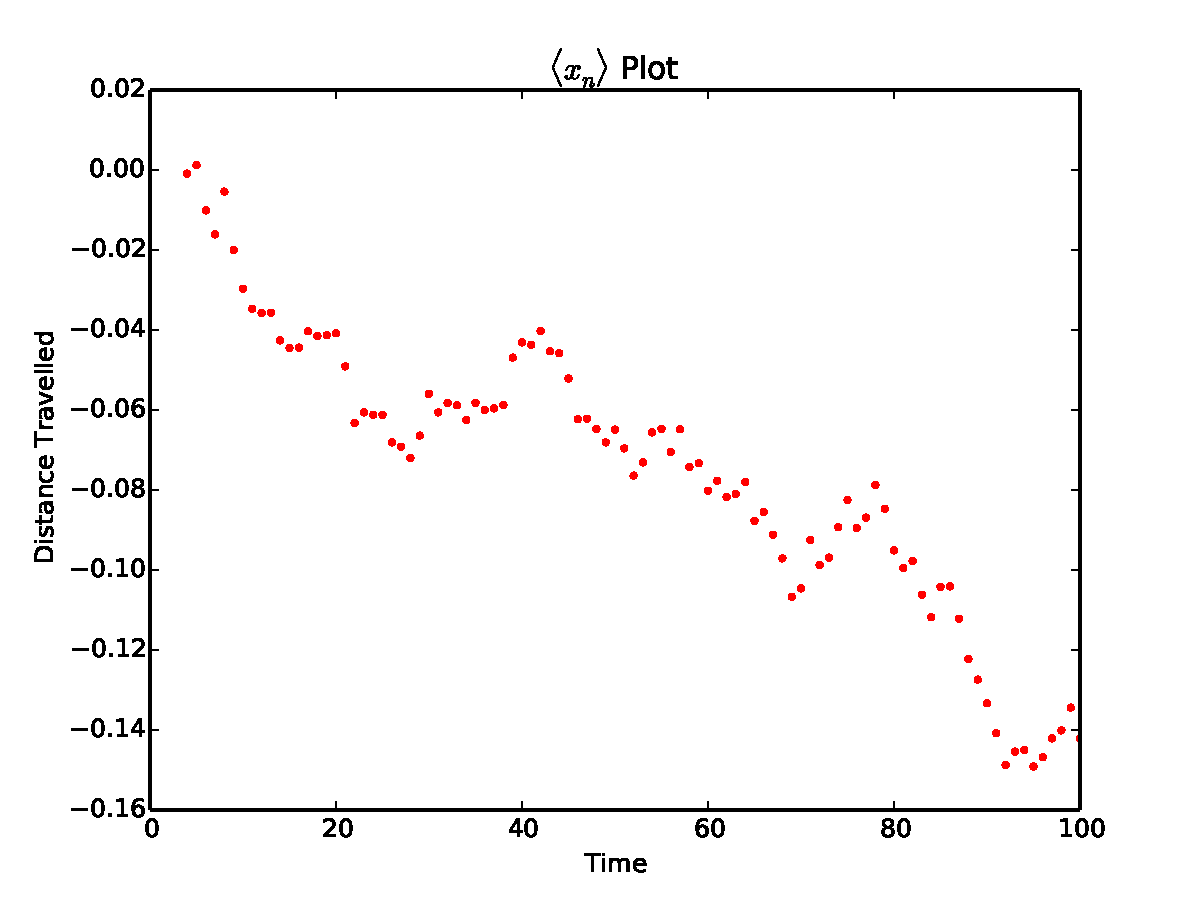
\includegraphics[width=.6\textwidth]{../output/plots_for_paper/problem_1/xn_Plot.pdf}
  	{\par\nobreak\rule[9pt]{35em}{0.5pt}\vspace{-5mm}}
	\caption{$\langle x_{n} \rangle$ plot}
	\label{fig:1_a_1}
  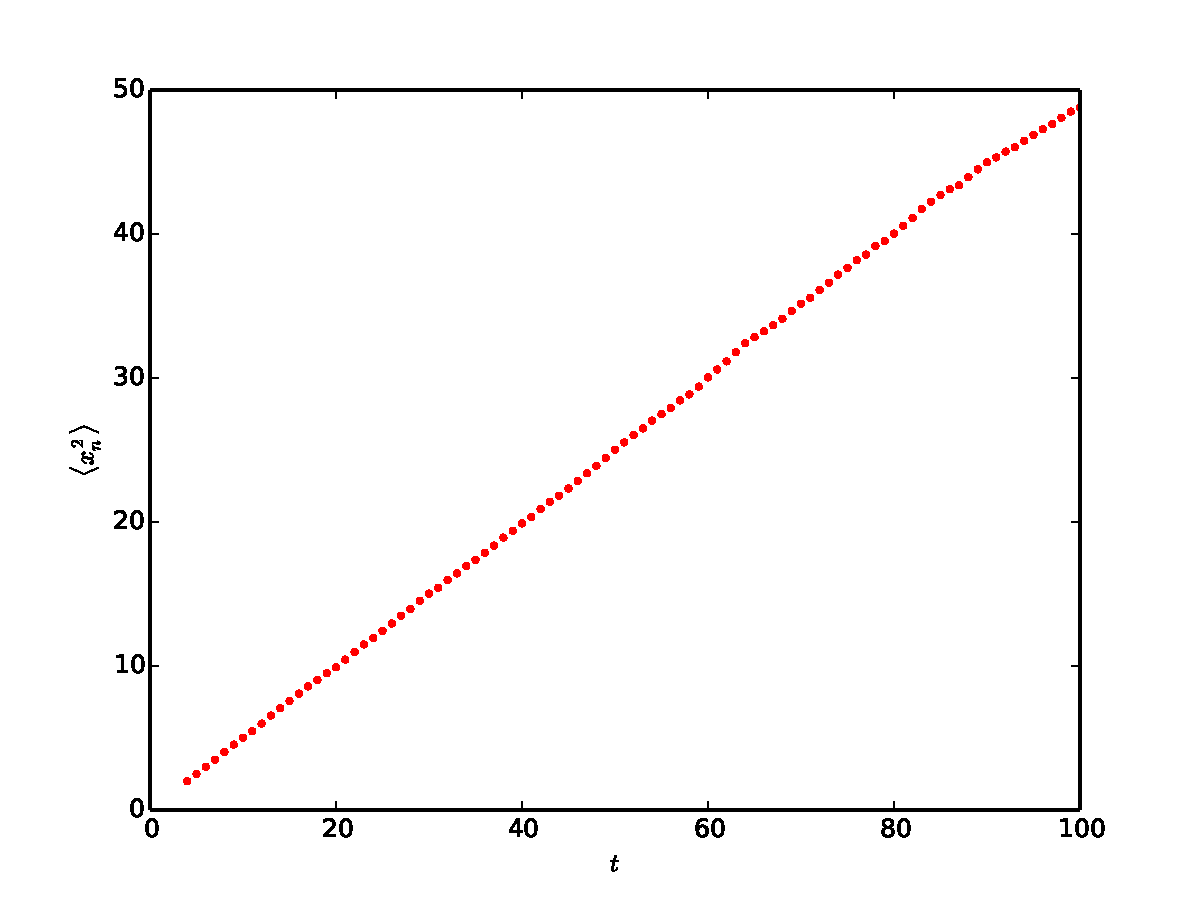
\includegraphics[width=.6\textwidth]{../output/plots_for_paper/problem_1/xn2_Plot.pdf}
  	{\par\nobreak\rule[9pt]{35em}{0.5pt}\vspace{-5mm}}
	\caption{$\langle x_{n}^{2} \rangle$ plot}
	\label{fig:1_a_2}
\end{figure}

\newpage

\subsubsection{Part B}
\begin{figure}[!htbc]
  \centering
  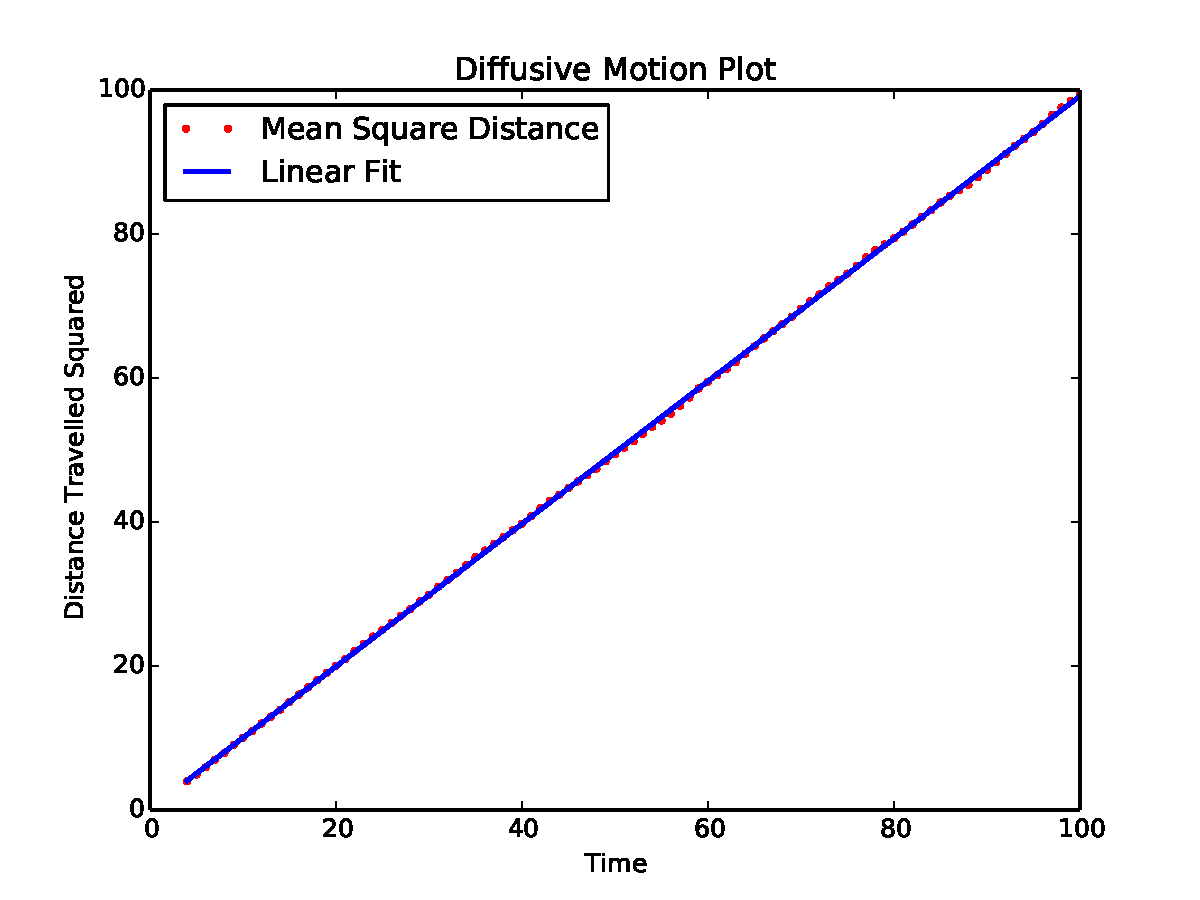
\includegraphics[width=.6\textwidth]{../output/plots_for_paper/problem_1/Diffusion_Plot.pdf}
  	{\par\nobreak\rule[9pt]{35em}{0.5pt}\vspace{-5mm}}
	\caption{Diffusive motion plot}
	\label{fig:1_b}
\end{figure}

\subsection{Diffusion Equation}
\label{subsec:results_2}
\subsubsection{Part a}
\label{subsubsec:results_2_a}
We derive the spatial expectation values $\expval{x^{2}(t)}$ as follows,
\begin{align}
	\expval{x^{2}(t)} &= \int_{-\infty}^{+\infty} \rho(x, t) x^{2} dx, \\
	\expval{x^{2}(t)} &= \frac{2}{\sqrt{2\pi\sigma^{2}(t)}} \int_{0}^{+\infty} x^{2} \exp(-\frac{x^{2}}{2\sigma^{2}(t)}).
\end{align}
Now we use the Gaussian integral that
\begin{equation}
	\int_{0}^{+\infty} x^{2n} \exp(-x^{2}/a^{2}) dx = \sqrt{\pi} \frac{(2n)!}{n!}\Big( \frac{a}{2} \Big)^{2n+1}.
\end{equation}
Let $n = 1$ and $a = \sqrt{2}\sigma(t)$, we can get
\begin{equation}
	\begin{split}
		\expval{x^{2}(t)} &= \frac{2}{\sqrt{2\pi\sigma^{2}(t)}} \cdot \sqrt{\pi}\cdot \frac{2!}{1!} \cdot \Big( \frac{\sqrt{2}\sigma(t)}{2} \Big)^{3} \\
		&= \sigma^{2}(t).
	\end{split} 
\end{equation}

\newpage
\subsubsection{Part b}
\label{subsubsec:results_2_b}
\begin{figure}[!htbc]
  \centering
  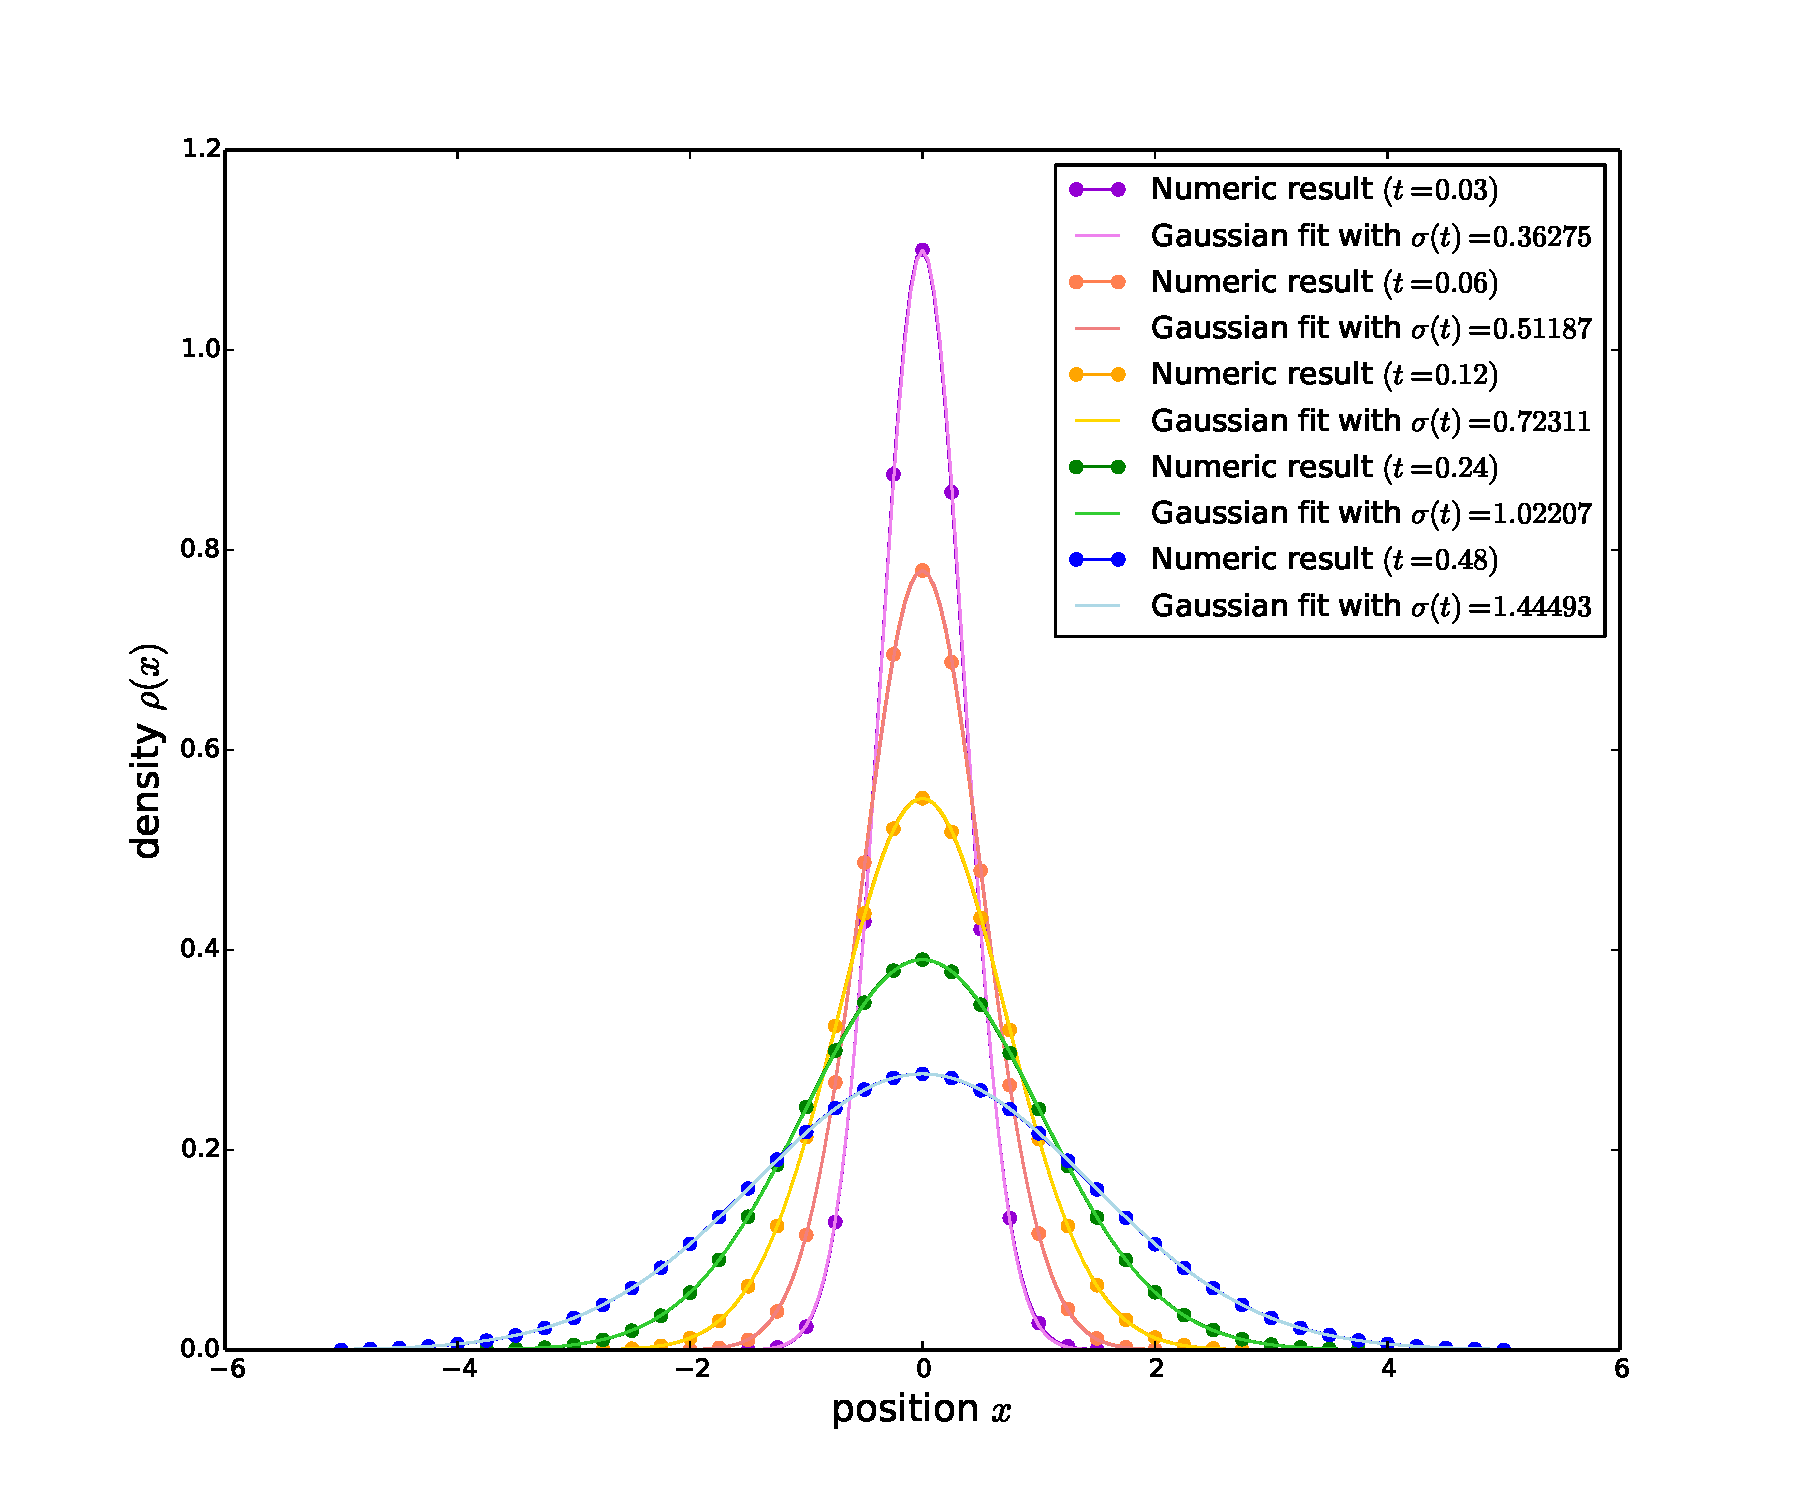
\includegraphics[width=.6\textwidth]{../output/plots_for_paper/problem_2/part_b.pdf}
  	{\par\nobreak\rule[9pt]{35em}{0.5pt}\vspace{-5mm}}
	\caption{Diffusion in one dimension}
	\label{fig:2}
\end{figure}

\begin{center}
	\begin{table}[!htbc]
		\begin{tabular}{ | p{2cm} | p{2cm} | p{2cm} | p{2cm} | p{2cm} |}
			\hline
			Steps & Time & $\sigma(t) = \sqrt{2Dt}$ & $\sigma_{\mathrm{fit}}(t)$ & Percent error\\
			\hline
			300  & 0.03 & 0.346 & 0.363 & 4.716\%\\
			\hline
			600  & 0.60 & 0.490 & 0.512 & 4.486\%\\ 
			\hline
			1200 & 1.20 & 0.693 & 0.723 & 4.371\%\\
			\hline
			2400 & 2.40 & 0.980 & 0.102 & 4.314\%\\
			\hline
			4800 & 4.80 & 0.139 & 0.144 & 4.279\%\\
			\hline
		\end{tabular}
		\caption{Theoretical data and fitting data}
		\label{table:prob_2}
	\end{table}
\end{center}

\clearpage
\subsection{Diffusion Limited Aggregation Model}
\label{subsec:results_3}
\begin{figure}[!h]
\centering
\subfigure[DLA cluster]
{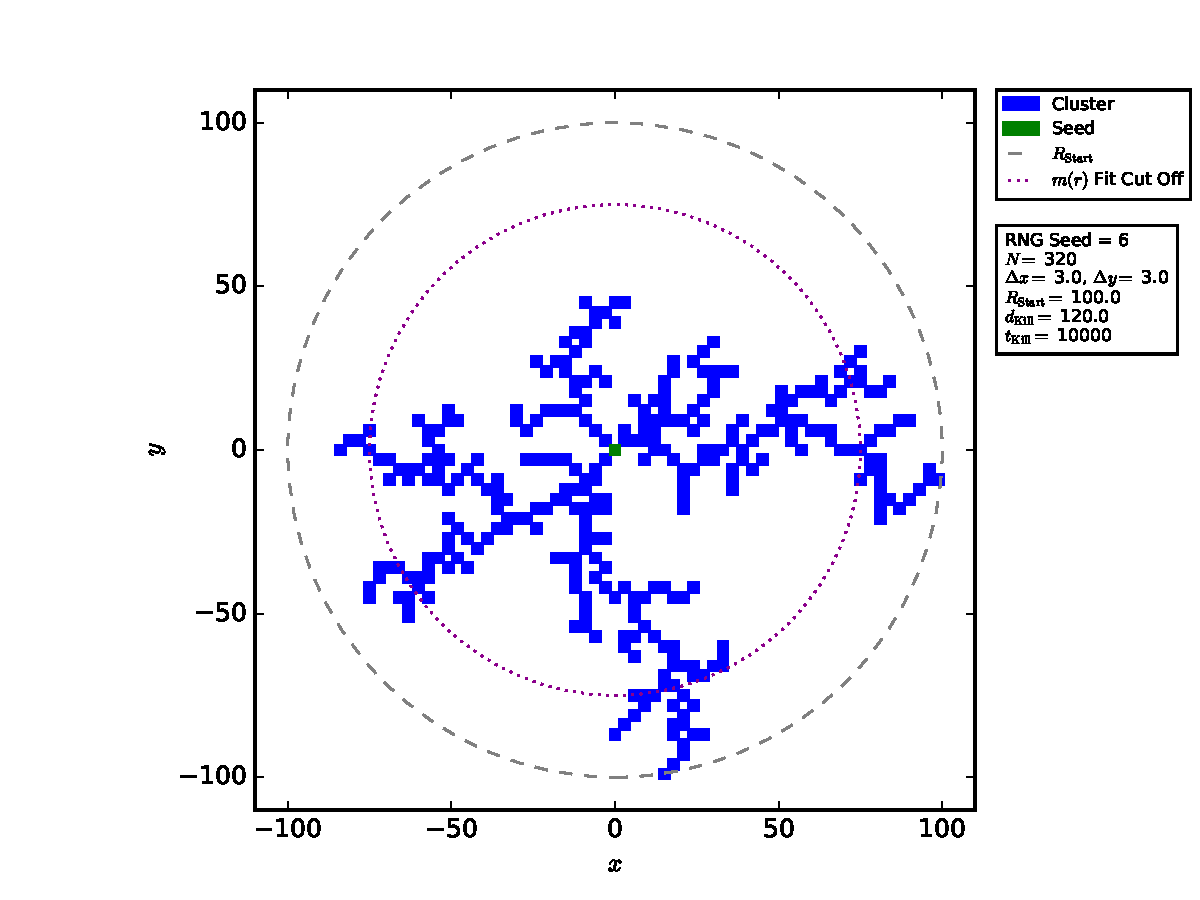
\includegraphics[width=3.4in]{../output/plots_for_paper/problem_3/large_cluster_seed_num_6.pdf}}
\subfigure[Fractal dimensionality extraction]
{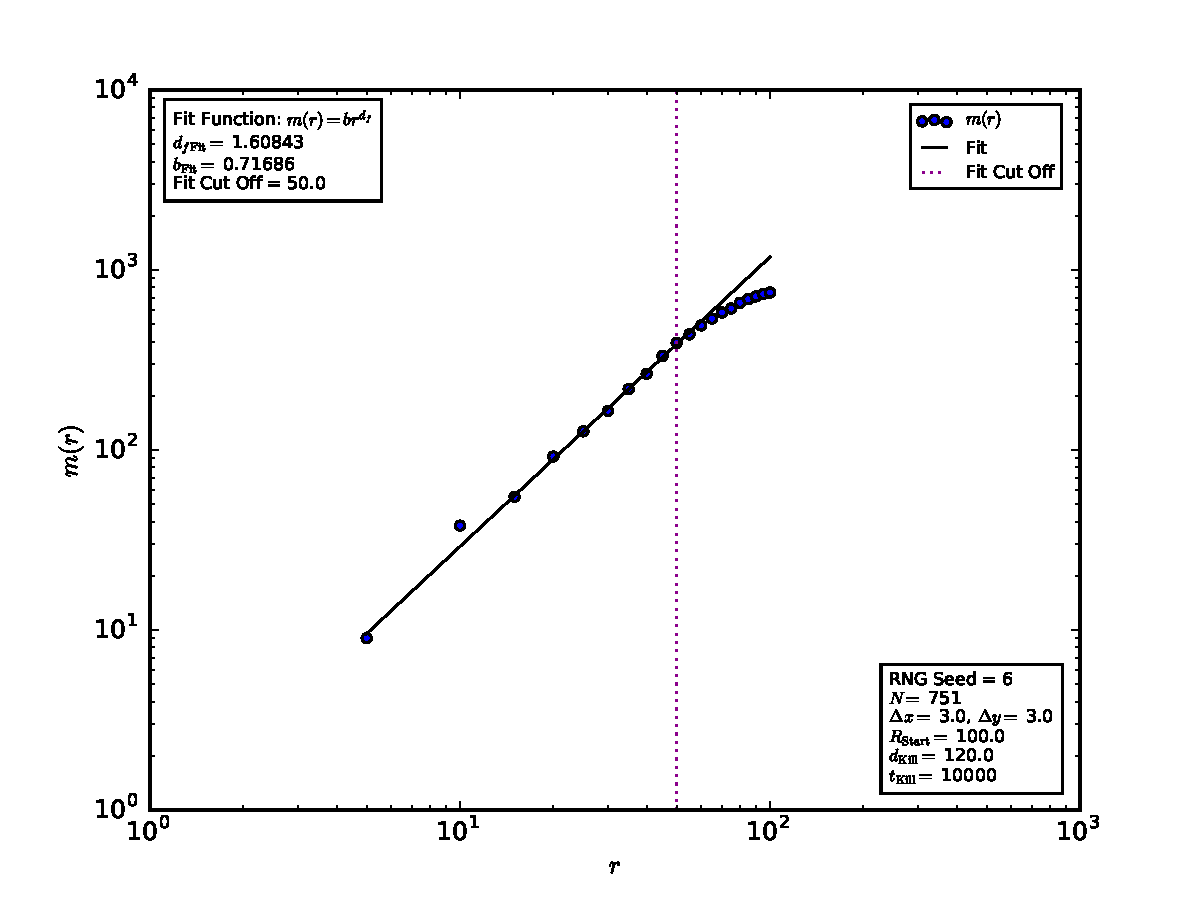
\includegraphics[width=3.4in]{../output/plots_for_paper/problem_3/large_cluster_mass_seed_num_6.pdf}}
\caption{DLA cluster representative sample I}
\label{dla1}
\end{figure}

\begin{figure}[!h]
\centering
\subfigure[DLA cluster]
{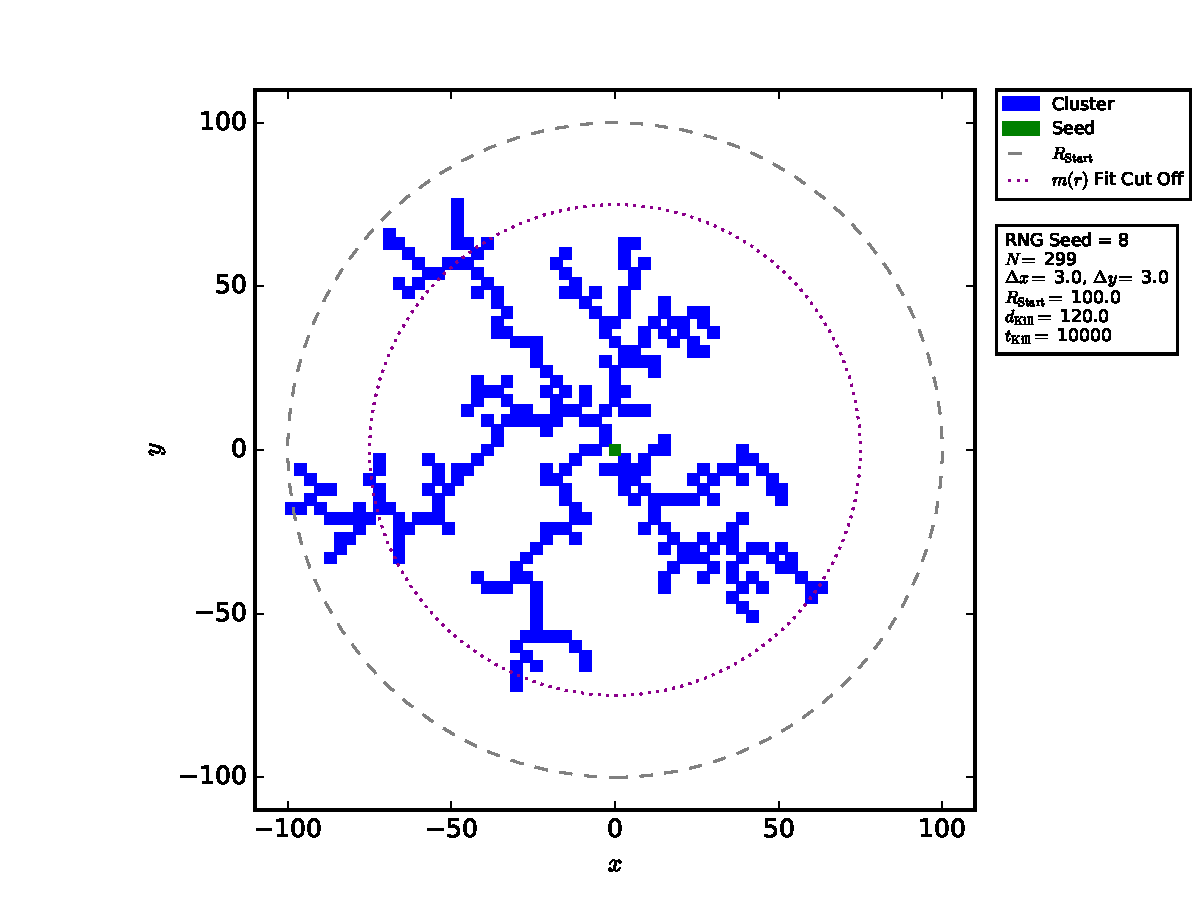
\includegraphics[width=3.4in]{../output/plots_for_paper/problem_3/large_cluster_seed_num_8.pdf}}
\subfigure[Fractal dimensionality extraction]
{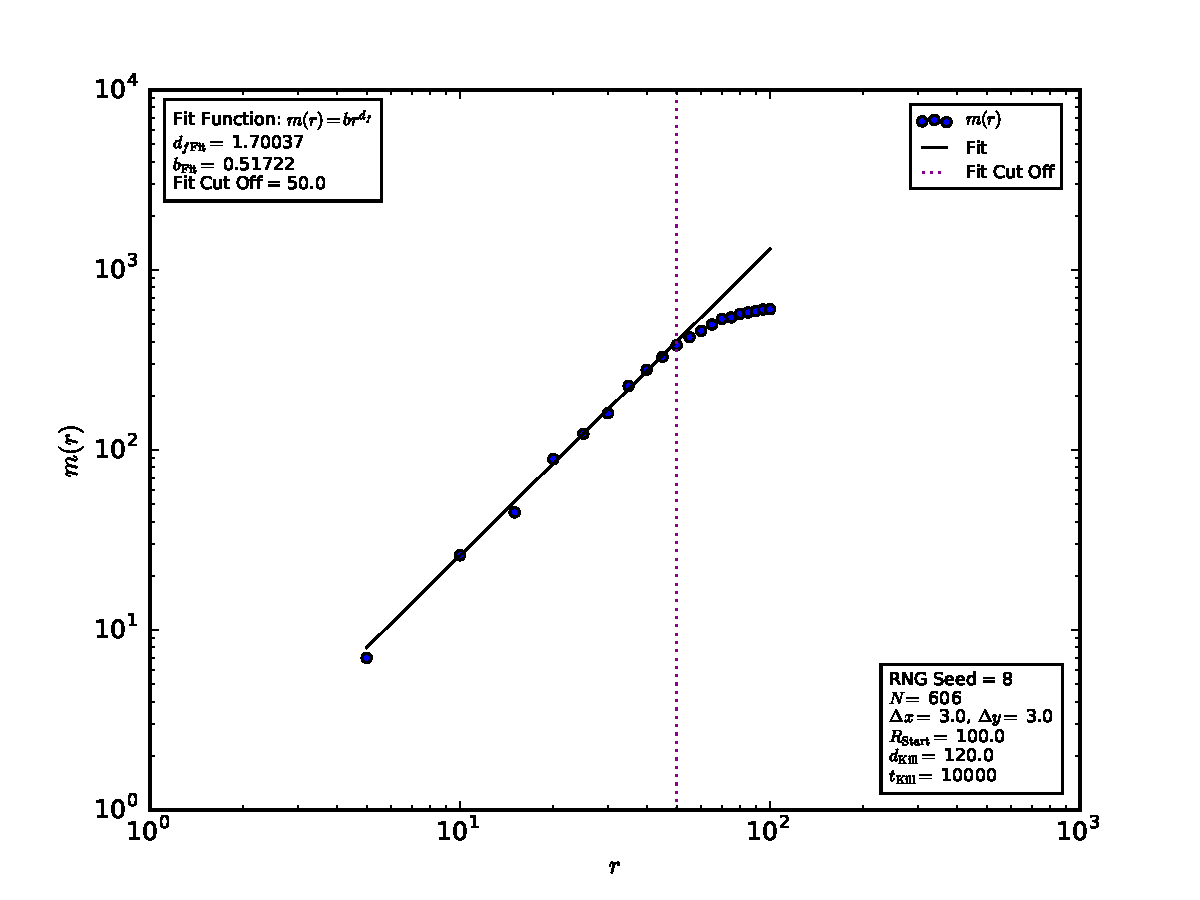
\includegraphics[width=3.4in]{../output/plots_for_paper/problem_3/large_cluster_mass_seed_num_8.pdf}}
\caption{DLA cluster representative sample II}
\label{dla2}
\end{figure}

\begin{figure}[!h]
\centering
\subfigure[DLA cluster]
{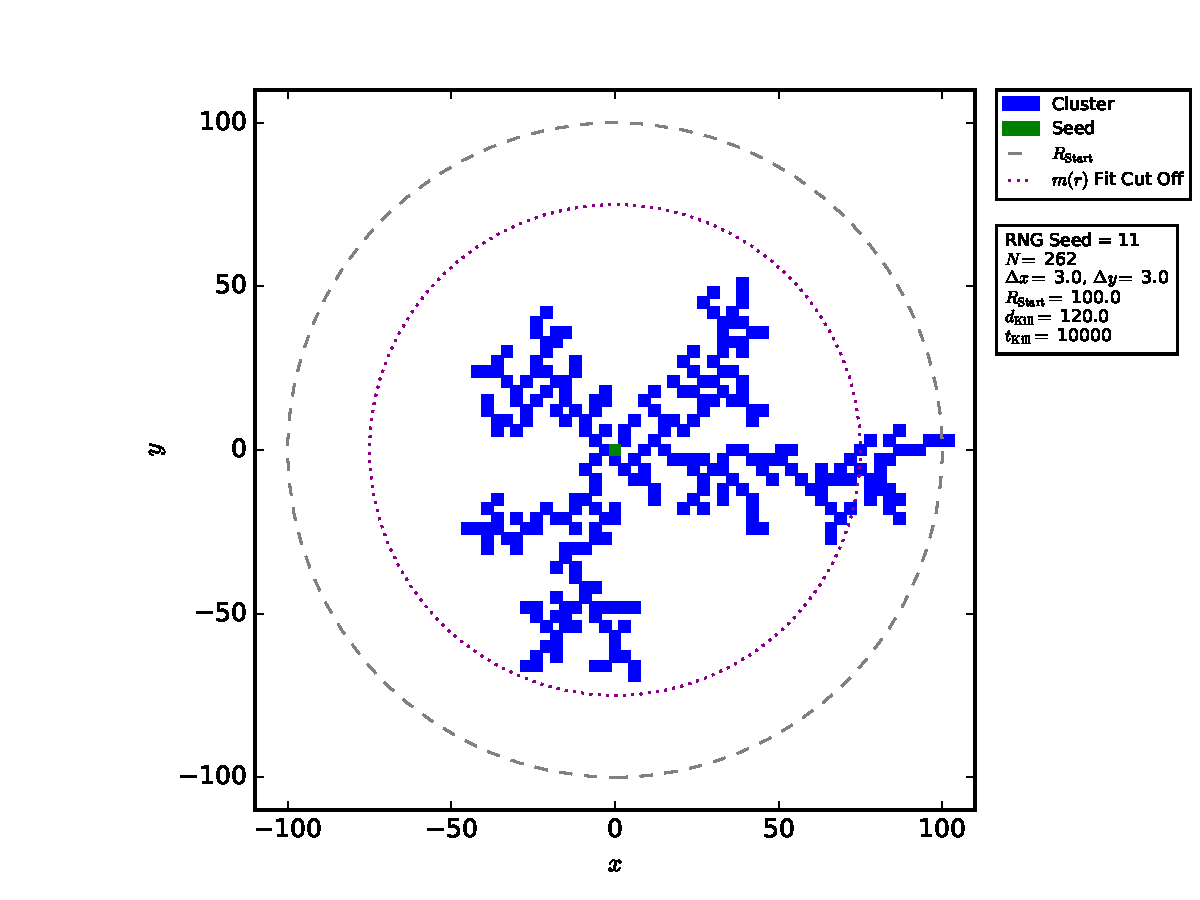
\includegraphics[width=3.4in]{../output/plots_for_paper/problem_3/large_cluster_seed_num_11.pdf}}
\subfigure[Fractal dimensionality extraction]
{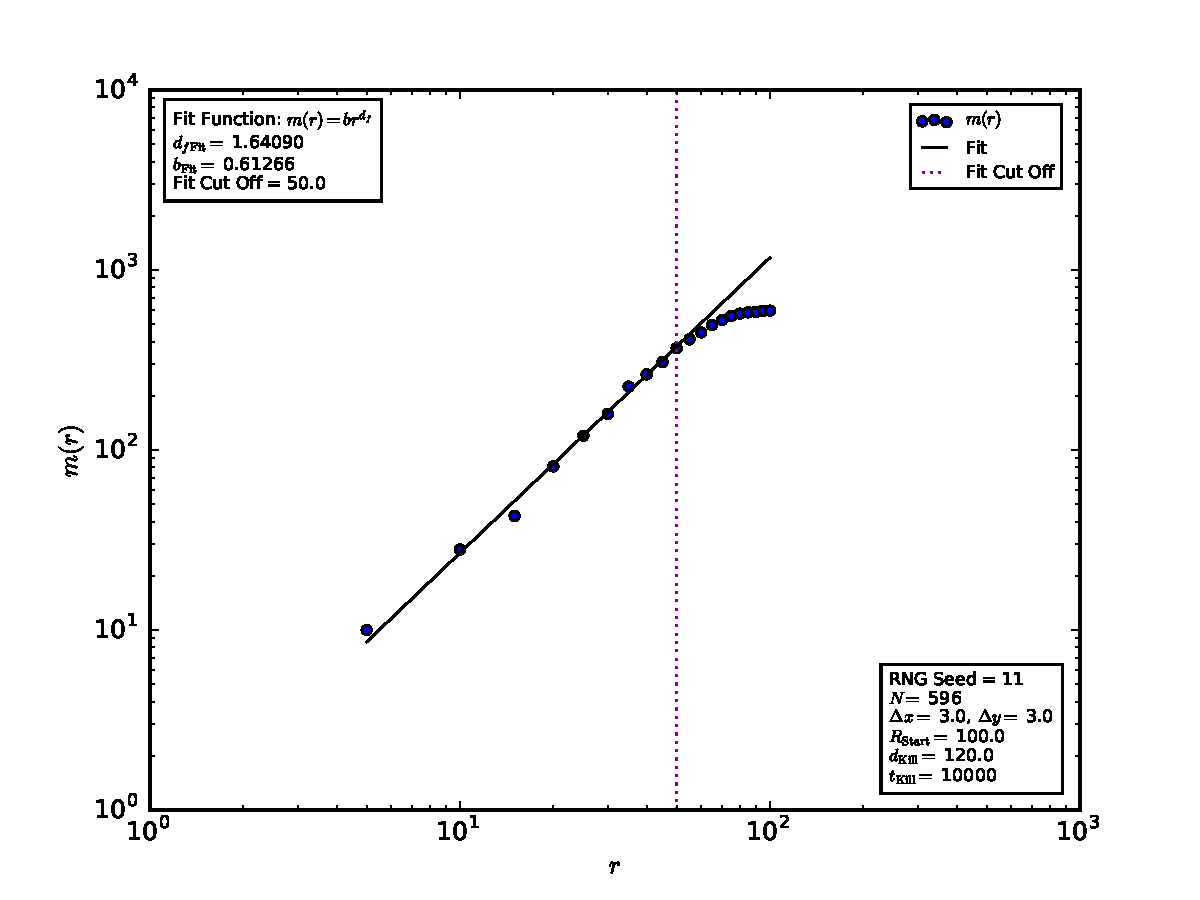
\includegraphics[width=3.4in]{../output/plots_for_paper/problem_3/large_cluster_mass_seed_num_11.pdf}}
\caption{DLA cluster representative sample III}
\label{dla3}
\end{figure}

\begin{figure}[!h]
\centering
\subfigure[DLA cluster]
{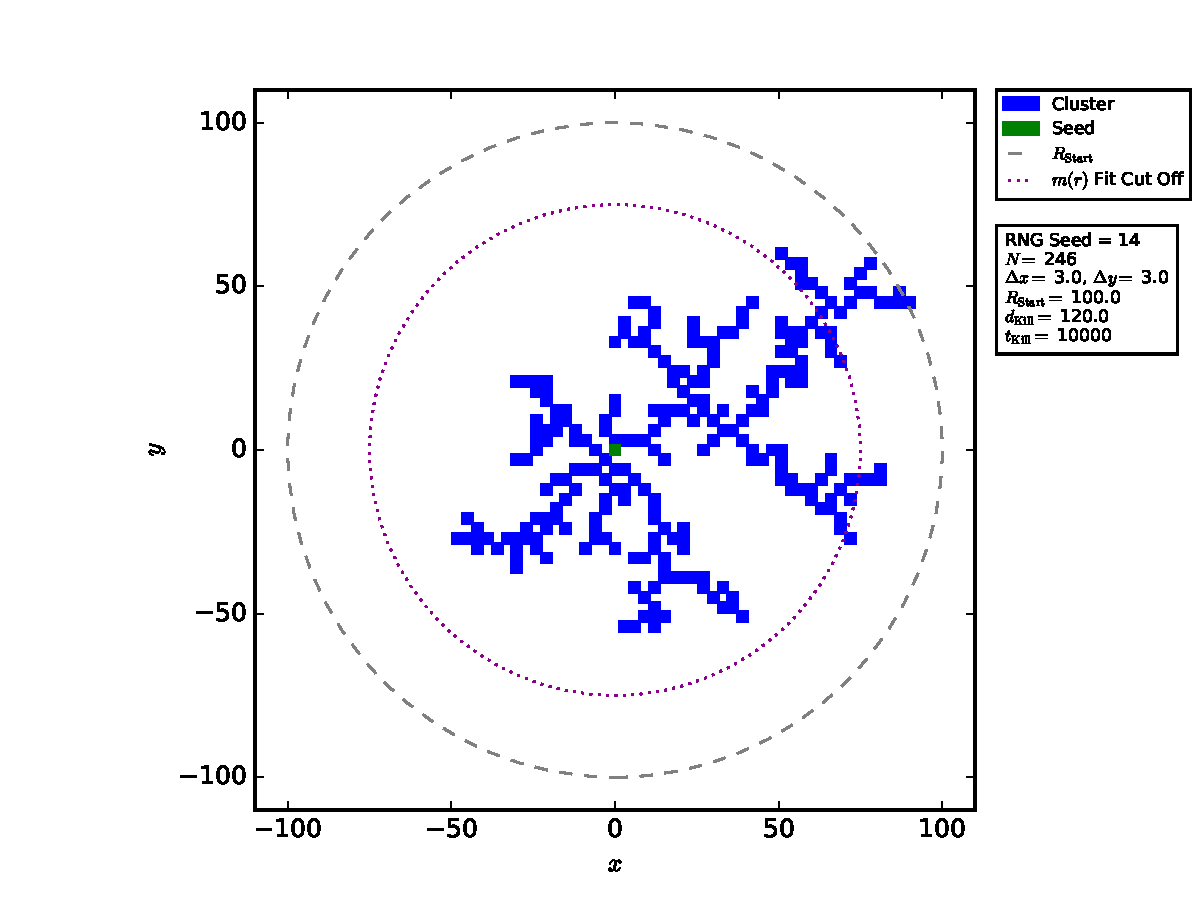
\includegraphics[width=3.4in]{../output/plots_for_paper/problem_3/large_cluster_seed_num_14.pdf}}
\subfigure[Fractal dimensionality extraction]
{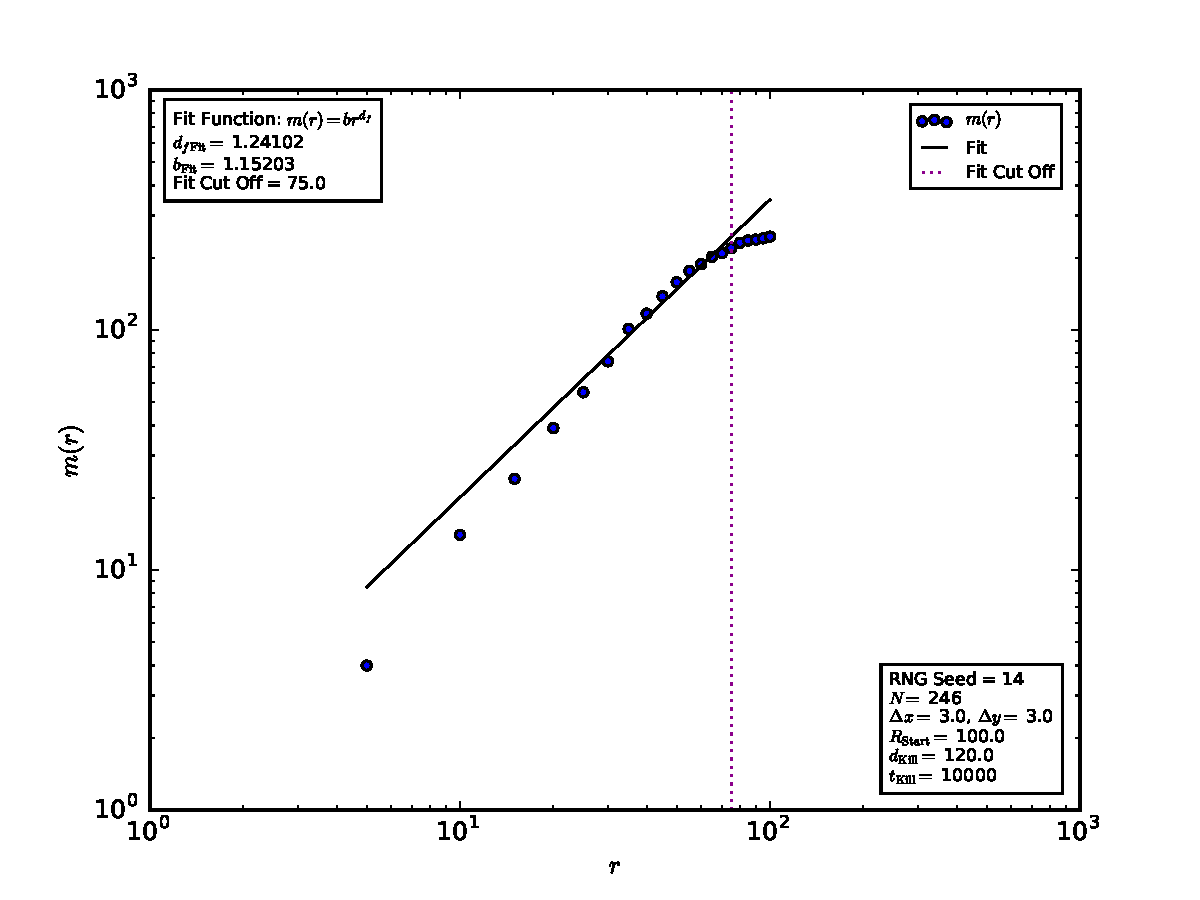
\includegraphics[width=3.4in]{../output/plots_for_paper/problem_3/large_cluster_mass_seed_num_14.pdf}}
\caption{DLA cluster representative sample IV}
\label{dla4}
\end{figure}


%%%%%%%%%%%%%%%%%%%% Discussion %%%%%%%%%%%%%%%%%%%%%%%%%%%%
\clearpage
\section{Discussion}
\label{sec:Conclusions}
\subsection{2D Random Walk}
In Fig.\ref{fig:1_a_1}, the average position of the walker looks to be around 0. The values fluctuate around 0 with a maximum value around 0.04 and a minimum value around -0.01. In Fig.\ref{fig:1_a_2}, the mean value of $x^2$ of the walker increases linearly with time and the slope of the graph is around 0.5.

In Part B, the results show that the relationship between distance traveled squared and time is linear. These results also show that the distance traveled square increases as time increases. By an ``eyeball" fit to the plot, we find the diffusion constant to be 0.25.

\subsection{Diffusion Equation}
As can be seen from the Fig.~\eqref{fig:2}, the numerical solutions coincide well with the analytic solutions. This figure also shows the evolution of a Gaussian pulse which gradually decreases in height and broadens in width. Table.~\eqref{table:prob_2} shows that $\sigma(t) = \sqrt{2Dt}$ and the percent error is around $4.5\%$. We can reduce the error by increasing the size of the boundary and decreasing the step size. Since the step size is limited by Eqn.~\eqref{eq:2_4}, it will be very time-consuming if we use smaller step size. 

\subsection{Cluster Growth with the DLA Model}
The graphs on the left hand side in Fig.\ref{dla1} - Fig.\ref{dla4} show 4 of the 10 cluster samples generated by the DLA model. The random walker starts from a random point on the dashed circle of radius 100. The seed is located at the origin and marked in green. The graphs on the right hand side plot $\log m$ versus $\log r$ and the fitting results for the fractal dimensionality. It is observed that the curves flatten out as $r$ gets larger. This is due to the finite size of the cluster. Thus we cut off the fitting at $r = R/2 = 50$ as is indicated by the dotted circles in the left graphs and the dotted vertical line in the right plots. 

By repeating the cluster growth procedure for 10 times using different random number generator seeds, we improve the accuracy in the fractal dimensionality extraction and get the mean value of $d_f$ to be 1.66 with a standard deviation of 0.14 (see the output log in Section \ref{sec:Supporting_Material}), which is consistent with the value given in class.



%%%%%%%%%%%%%%% Supporting Material %%%%%%%%%%%%%%%%%%%%%%%%
\clearpage
\section{Supporting Material}
\label{sec:Supporting_Material}

% insert the code's output, if it has useful information
\lstinputlisting[style=output,label={lst:output}]{../output/dla_log_output.log} 

The Python source code used to produce these results can be found online at \url{http://github.com/mepland/PHYS_566_Computational_Group_Project_1}, and is included in Section~\ref{sec:code}.
\clearpage
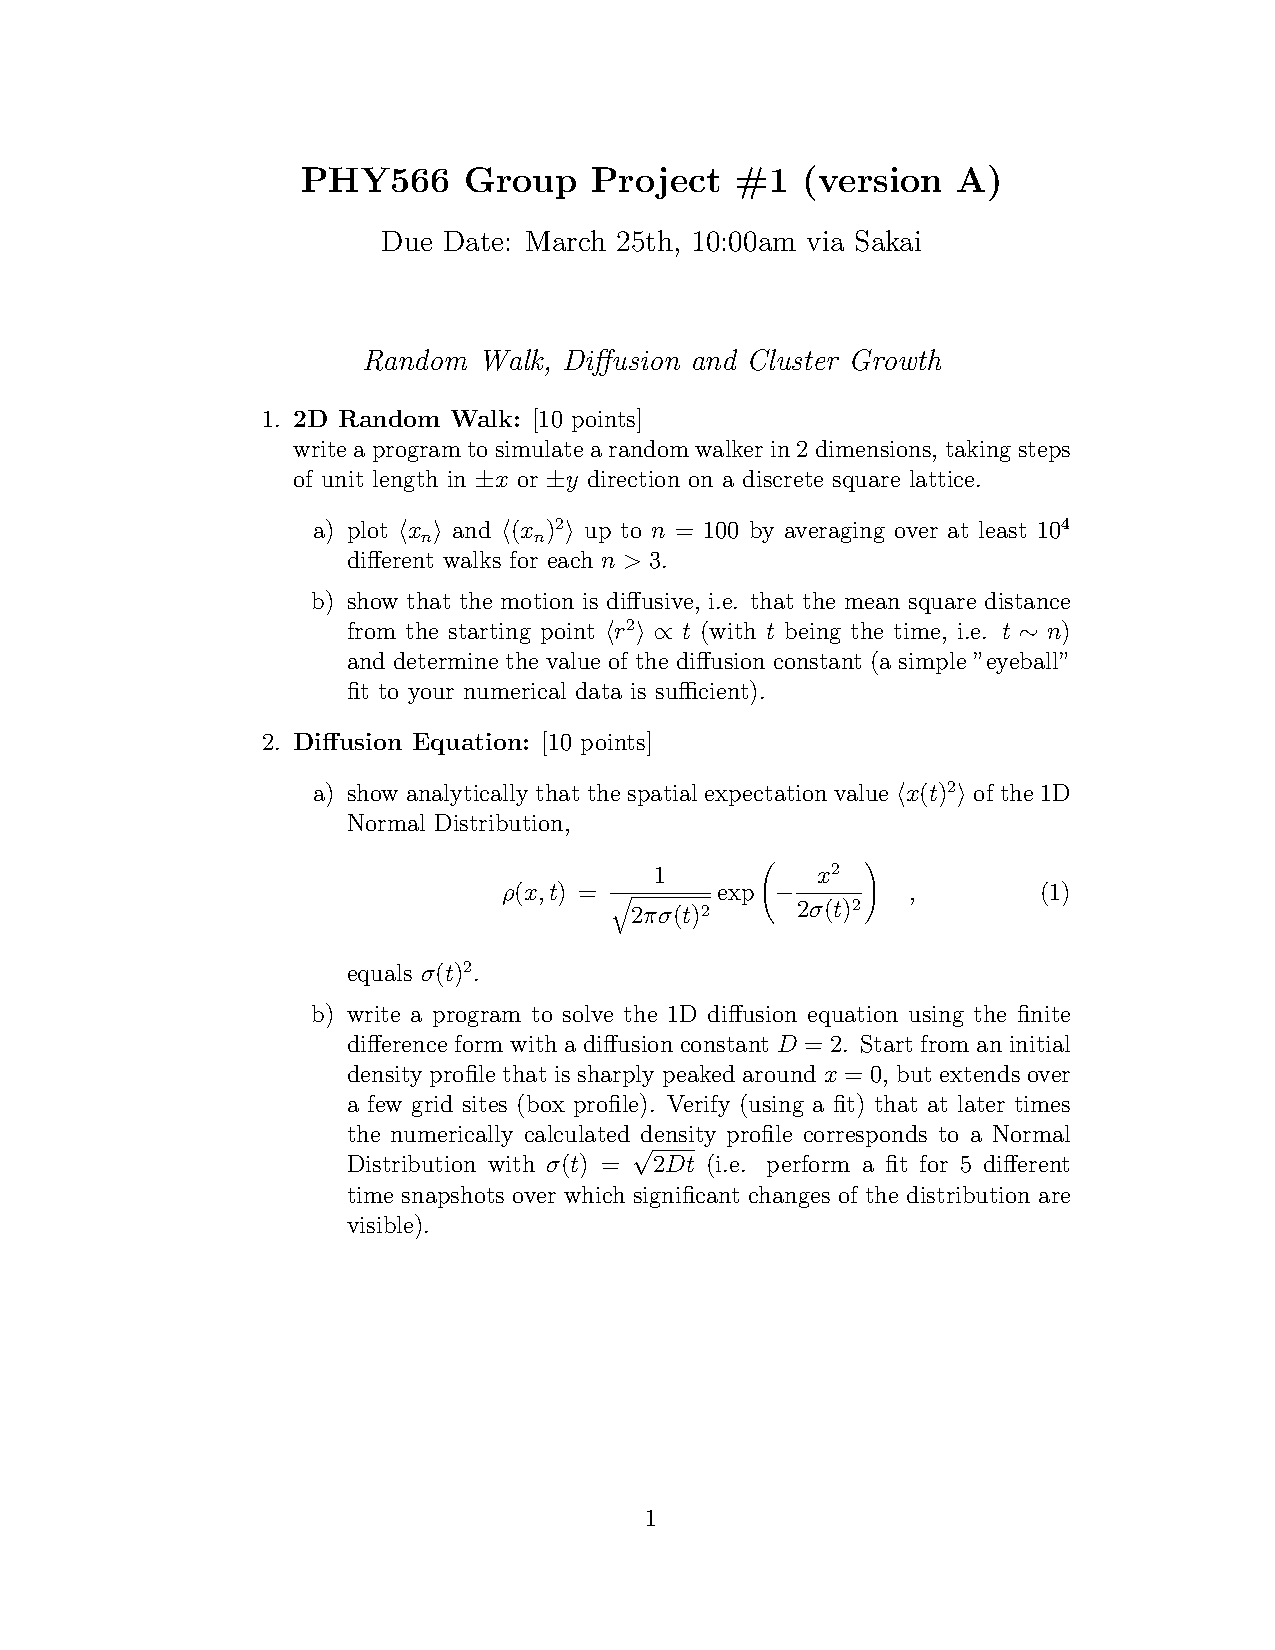
\includepdf[pages={1}]{../group_project1a.pdf}
\includepdf[pages={2}]{../group_project1a.pdf}

\clearpage
\section{Code}
\label{sec:code}

\lstinputlisting[style=python]{../code/2D_random_walk.py}

%\clearpage
\lstinputlisting[style=python]{../code/diffusion_eqn.py}

\clearpage
\lstinputlisting[style=python]{../code/dla.py}

\end{document} %%% end of doc %%%
%%%%%%%%%%%%%%%%%%%%%%%%%%%%%%%%%%%%%%%%%%%%%%%%%%%%%


\bibliographystyle{../bib_files/atlasBibStyleWoTitle}
\bibliography{../bib_files/my_bib.bib}

% Code to insert figures
\begin{figure}[!htbc]
  \centering
  \includegraphics[width=.6\textwidth]{part_a/TODO.pdf}
	{\par\nobreak\rule[9pt]{35em}{0.5pt}\vspace{-5mm}}
	\caption{TODO}
	\label{fig:TODO}
\end{figure}

